\documentclass[10pt,twocolumn,letterpaper]{article}

\usepackage{cvpr}
\usepackage{times}
\usepackage{epsfig}
\usepackage{graphicx}
\usepackage{amsmath}
\usepackage{amssymb}

% Include other packages here, before hyperref.

% If you comment hyperref and then uncomment it, you should delete
% egpaper.aux before re-running latex.  (Or just hit 'q' on the first latex
% run, let it finish, and you should be clear).
\usepackage[pagebackref=true,breaklinks=true,letterpaper=true,colorlinks,bookmarks=false]{hyperref}

\cvprfinalcopy % *** Uncomment this line for the final submission

\def\cvprPaperID{****} % *** Enter the CVPR Paper ID here
\def\httilde{\mbox{\tt\raisebox{-.5ex}{\symbol{126}}}}

% Pages are numbered in submission mode, and unnumbered in camera-ready
\ifcvprfinal\pagestyle{empty}\fi
\begin{document}

%%%%%%%%% TITLE
\title{Project Report : CS 7643}

\author{First Author, Second Author, Karan Vohra, Qimeng Wu\\
Georgia Institute of Technology\\
{\tt\small firstauthor@i1.org}, {\tt\small secondauthor@i2.org}, {\tt\small third@i2.org}, {\tt\small kvohra3@gatech.edu}, {\tt\small  qimeng@gatech.edu}
% For a paper whose authors are all at the same institution,
% omit the following lines up until the closing ``}''.
% Additional authors and addresses can be added with ``\and'',
% just like the second author.
% To save space, use either the email address or home page, not both
}
\maketitle
%\thispagestyle{empty}

%%%%%%%%% ABSTRACT
\begin{abstract}
   The experience of seeing a food dish and wanting to know how to create it yourself is something almost every person can relate towards. Especially with the addition of social media to our daily life, people are constantly fed pictures of mouth-watering dishes. Getting a taste of these dishes may not be feasible, but thanks to the increase in classification technologies there is potential for a user to be able get the recipe for any dish they see and be able to recreate it themselves. In order to accomplish this goal we implement a model that utilizes a deep convolutional neural network that classify food images into categories and cooking techniques in order to output a matching recipe using a nearest neighbor model. In this report, we explain the model setups, showcase the benefits and challenges faced, walk through the experiment setup, and analyze the results recieved from each model and the overall network. 
\end{abstract}

%%%%%%%%% BODY TEXT
\section{Introduction/Background/Motivation}

(5 points) What did you try to do? What problem did you try to solve? Articulate your objectives using absolutely no jargon. 

(5 points) How is it done today, and what are the limits of current practice?

(5 points) Who cares? If you are successful, what difference will it make? 

(5 points) What data did you use? Provide details about your data, specifically choose the most important aspects of your data mentioned \href{https://arxiv.org/abs/1803.09010}{here}. You don’t have to choose all of them, just the most relevant.
(5 points) What did you try to do? What problem did you try to solve? Articulate your objectives using absolutely no jargon. 

(5 points) How is it done today, and what are the limits of current practice?

(5 points) Who cares? If you are successful, what difference will it make? 

(5 points) What data did you use? Provide details about your data, specifically choose the most important aspects of your data mentioned \href{https://arxiv.org/abs/1803.09010}{here}. You don’t have to choose all of them, just the most relevant.
(5 points) What did you try to do? What problem did you try to solve? Articulate your objectives using absolutely no jargon. 

(5 points) How is it done today, and what are the limits of current practice?

(5 points) Who cares? If you are successful, what difference will it make? 

(5 points) What data did you use? Provide details about your data, specifically choose the most important aspects of your data mentioned \href{https://arxiv.org/abs/1803.09010}{here}. You don’t have to choose all of them, just the most relevant.
(5 points) What did you try to do? What problem did you try to solve? Articulate your objectives using absolutely no jargon. 

(5 points) How is it done today, and what are the limits of current practice?

(5 points) Who cares? If you are successful, what difference will it make? 

(5 points) What data did you use? Provide details about your data, specifically choose the most important aspects of your data mentioned \href{https://arxiv.org/abs/1803.09010}{here}. You don’t have to choose all of them, just the most relevant.
(5 points) What did you try to do? What problem did you try to solve? Articulate your objectives using absolutely no jargon. 

(5 points) How is it done today, and what are the limits of current practice?

(5 points) Who cares? If you are successful, what difference will it make? 

(5 points) What data did you use? Provide details about your data, specifically choose the most important aspects of your data mentioned \href{https://arxiv.org/abs/1803.09010}{here}. You don’t have to choose all of them, just the most relevant.
(5 points) What did you try to do? What problem did you try to solve? Articulate your objectives using absolutely no jargon. 

(5 points) How is it done today, and what are the limits of current practice?

(5 points) Who cares? If you are successful, what difference will it make? 

(5 points) What data did you use? Provide details about your data, specifically choose the most important aspects of your data mentioned \href{https://arxiv.org/abs/1803.09010}{here}. You don’t have to choose all of them, just the most relevant.

%-------------------------------------------------------------------------
%------------------------------------------------------------------------
\section{Approach}
\begin{figure*}
\begin{center}
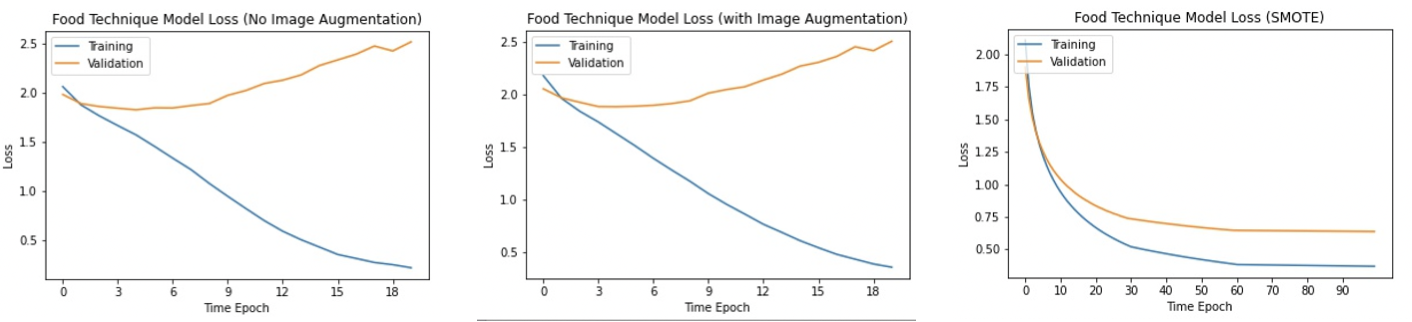
\includegraphics[width=1.0\linewidth]{technique_model_loss_curve}
\end{center}
  \caption{Technique Loss Curves.}
\label{fig:loss_curve}
\end{figure*}

\begin{table*}
\begin{center}
\begin{tabular}{|c|l|l|l|l|l|l|l|l|l|l|}
\hline
 & bake & braise/stew & chill & fry & grill/broil & marinate & moist-heat & no-cook & roast & saute \\
\hline\hline
Raw Image & 0.7192 & 0.0563 & 0.2143 & 0.1575 & 0.2408 & 0.0625 & 0.1157 & 0.1319 & 0.2739 & 0.25 \\
With Augmentation & 0.6229 & 0.31 & 0.3846 & 0.2533 & 0.2402 & 0.2674 & 0.2057 & 0.411 & 0.1931 & 0.1825 \\
With SMOTE & 0.9663 & 0.8066 & 0.8492 & 0.8544 & 0.9145 & 0.8034 & 0.9721 & 0.772 & 0.7572 & 0.5073 \\
\hline
\end{tabular}
\end{center}
\caption{Technique Accuracy Comparison.}
\label{tab:accuracy}
\end{table*}
Our application is solving the problem of returning a possible recipe given an input image of a food dish. The original dataset contains all the food images and associated recipes needed to train our model. In order to solve this problem, our application takes a query approach. Given an input image, we find the top five similar images and then return the recipes of these top five images. As work on this project progressed, our definition of 'similar' evolved. It started with us querying images that looked similar. While this initial - and trivial - approach worked great for some foods, it would often run into the issue of associating two dishes that looked similar but in reality were complete different. In order to combat this and improve our query results, we looked to upgrade our network. Instead of utilizing just a basic nearest neighbour model to find similar looking images we also built two additional models - one to predict food categories and one to predict the cooking technique.
\subsection{Image Feature Extraction}
The base model we use to extract image features is VGG16 \cite{Authors01}. It has a feature layer composed by a set of convolution layers and max pooling layers, an average pooling layers and a classification layer which is composed by three fully connected layers, ReLU activation layers and drop out layers. 
The parameters of the feature layer in the network are frozen. We are updating the parameters in the fully connected layers to do predictions for the food technique and categories. When we use VGG16 to do image feature extractions, we dropped the last layer that was originally used to do 1000-way ILSVRC classification. Then, for each input image, we first resize it to 256x256, do a centre crop with size 224, and then feed it into the network. The result is a feature vector with dimension 4096 for each input image.
\subsection{Nearest Neighbour}
Our nearest neighbor implementation is straight forward. We extract features from image in our over 13,000+ images dataset using the VGG16 network.
We then extract the feature from the input image as well. A cosine similarity is calculated on the input image and each image in the dataset. The images with the top five similarities are taken and the recipes are output.
\subsection{Food Technique}
The original dataset does not come label the images with the techniques. In order to gather this information, 8600 images with technique labels was scraped from the same website, Epicurious. The effort generated 20 total unbalanced techniques. A few steps were taken to mitigate this problem. First a consolidation of techniques was done. For example, techniques such as “fry”, “pan-fry”, “stir-fry”, and “deep-fry” were all consolidated in "fry". This effort was able to cut down the number of techniques from 20 to 10, giving the minority classes much more representation than before. However, the majority classes also gained the same benefit and had about five times the representation as the minority class. Two different methods were used to correct this issue. 

The first approach was to perform some image augmentation on for images in the minority classes. Augmentation was performed so minority classes would have equal representation as the majority class. We overwrite the original VGG16’s last classification layer to have 10 classes at the end and froze the feature layers to build this technique prediction model.

The second approach was to use the similar feature extraction method (nearest neighbour) for all the images and then use SMOTE\cite{Authors02} to oversample the minority classes' features. As for the model, we just built a simple one linear layer model that takes the feature vector with dimension 4096 and output 10 dimensions.

Another approach we tried is to use the similar feature extraction method, as in nearest neighbour, for all the images and then we use SMOTE \cite{Authors02} to oversample minority classes’ features. As for the model, we just built a simple one linear layer model that takes the feature vector with dimension 4096 and output 10 dimensions.
\begin{table}
\begin{center}
\begin{tabular}{|l|c|}
\hline
Technique & Count \\
\hline\hline
bake & 2756 \\
grill/broil &  993 \\
saute &  880 \\
roast &  827 \\
chill &  709 \\
fry &  661 \\
moist-heat-cooking &  637 \\
no-cook &  401 \\
braise/stew &  314 \\
marinate &  270 \\
\hline
\end{tabular}
\end{center}
\caption{Techniques Count}
\label{tab:techniques_count}
\end{table}

\subsection{Food Category}
Similar to the food technique model, the original dataset did not contain any category label for each food dish. In order to generate categories for each image, we implement the Latnent Dirichlet Allocation(LDA) approach to topic modeling. The topic modeling algorithm is outside the scope of this paper, so only a high level overview will be given here\cite{Authors03}. A deeper dive can be found in the paper linked in the References sections. Topic modeling is a type of statically model that is utilized to discover specific "topics" found within a dataset. In our approach we preprocess our data by abstracting out the titles from our dataset by tokenizing and lemmatize each title. This process cleans up the titles to be in the same casing, removing extra symbols or tokens that are too short, and removes any inflectional endings that can be found in the title (i.e. 'roasted' will become 'roast'). After the data has been cleaned, we incorporate a NMF embedding which generates our 30 unique categories. 

During the initial stages, the topic model was generating 200 unique categories and assigned each image with the best matched category. However, this resulted in majority of our categories not containing a significant amount of images. As a result, this implementation generated abysmal results. After training for 50 epochs and using cross entropy as our loss function, all the categories except one were scoring 0.0. The data set was heavily unbalanced and was resulting in the model severely over fitting to be able to only correctly identify one category. The loss function was updated to start utilizing focal loss in order to combat the class imbalance, but no improvement was being seen. 

In order to mitigate this issue the topic model was adjusted to bucket each image in 30 unique categories. This allowed for more generic labels and allowed the model to perform better across all categories. Furthermore, in order to compensate for the unbalanced categories we also implement SMOTE to over sample the minority categories. The model utilizes the same linear layer model used within the technique model that takes an input dimension of 4096 and outputs a dimension of 10. This approach coupled with continuing to use focal loss as the loss function, showed the best results. However, even these results were deemed to be inadequate and potential detrimental to the overall accuracy of the network. 

\section{Experiments and Results}
\begin{table*}
\begin{center}
\begin{tabular}{|c|l|l|l|l|}
\hline
 & Train Accuracy Mean & Train Accuracy Final & Validation Accuracy Mean & Validation Accuracy Final \\
\hline\hline
Cross Entropy Loss (200 categories) & 0.8544 & 0.9981 & 0.2824 & 0.2635 \\
Cross Entropy Loss (30 categories) & 0.8545 & 0.9979 & 0.2907 & ? \\
Focal Loss (30 categories) & 0.8225 & 0.9972 & 0.2671 & 0.3017 \\
\hline
\end{tabular}
\end{center}
\caption{Category Accuracy Comparison}
\label{tab:category_accuracy}
\end{table*}

\begin{table}
\begin{center}
\begin{tabular}{|l|c|c|}
\hline
Category & CE Loss & Focal Loss \\
\hline\hline
Class 0 & 0.0435 & 0.0959 \\
Class 1 & 0.1833 & 0.1190 \\
Class 2 & 0.2775 & 0.4012 \\
Class 3 & 0.0690 & 0.0543 \\
Class 4 & 0.0943 & 0.1831 \\
Class 5 & 0.1209 & 0.0568 \\
Class 6 & 0.0000 & 0.0000 \\
Class 7 & 0.2151 & 0.1753 \\
Class 8 & 0.0734 & 0.1262 \\
Class 9 & 0.0794 & 0.0492 \\
Class 10 & 0.0658 & 0.09303 \\
Class 11 & 0.0000 & 0.00003 \\
Class 12 & 0.0676 & 0.05713 \\
Class 13 & 0.2821 & 0.12963 \\
Class 14 & 0.0182 & 0.01853 \\
Class 15 & 0.0484 & 0.03703 \\
Class 16 & 0.1111 & 0.06763 \\
Class 17 & 0.0190 & 0.04493 \\
Class 18 & 0.1667 & 0.07953 \\
Class 19 & 0.0615 & 0.00003 \\
Class 20 & 0.1667 & 0.19303 \\
Class 21 & 0.1000 & 0.09723 \\
Class 22 & 0.0392 & 0.01793 \\
Class 23 & 0.0685 & 0.05883 \\
Class 24 & 0.0152 & 0.01753 \\
Class 25 & 0.0902 & 0.09853 \\
Class 26 & 0.0600 & 0.02303 \\
Class 27 & 0.0862 & 0.02173 \\
Class 28 & 0.0455 & 0.04443 \\
Class 29 & 0.3324 & 0.48093 \\
\hline
\end{tabular}
\end{center}
\caption{Per Category Accuracy Comparison}
\label{tab:per_category_accuracy}
\end{table}


\subsection{Food Technique Classification}
Due to the fact that the data set is imbalanced, we are using the per class accuracy in conjunction with the top-3 accuracy in order to measure the performance in the technique classification model. The number of images in the data set found in each class bucket can be found in Table \ref{tab:techniques_count}. As the seen in Table \ref{tab:accuracy}, the model is able to perform well on majority classes (i.e 'bake'), but is not able to translate that to he minority classes (i.e. 'braise/stew' or 'marinate'). Intuitively, this is most likely because the model does not have enough images in the minority classes for it to draw meaningful connections. We can prove this further when looking at the accuracy history while the model trains. The minority classes all start with an accuracy of 0,but gradually increase as the number of epochs increase and the model sees more images with the minoirty class labels. Furthermore, when image augmentation was applied to equalize the distribuiton across class labels, the model was able to improve its per class accuracy. 

However, as you can see from the loss curves in Figure  \ref{fig:loss_curve}, training with both raw images and augmented images tend to have overfitting issues. We are using cross-entropy loss function and Adam as the optimizer. We did try using a smaller learning rate, a larger regularization term or even switch the optimizer to SGD, but as it turned out, it would just slow down the process to reach the elbow point of the validation loss curve instead of making any progress minimizing the loss. \\

What we thought the bottleneck at this point is that the the performance on the minor classes are still not good and not able to improve further. Though augmentation helped a bit, it is still not able to solve the issue. We think this is probably related to the fact that technique is not a physical object. So, the image augmentation method that does the rotation, random crop, flip or blurring doesn’t actually add that much new information needed for technique classification. \\
Then, we tried SMOTE, which we use to oversample the data through images’ feature space extracted from the VGG16 network. This turned out to be able to add in much more useful new information for the model to learn about the minor technique classes. We achieved a 93.47\% top-3 accuracy and the per class accuracy improves a lot as well. Meanwhile, we don’t have the elbow point in the validation loss curve anymore. Both training and validation loss curves are able to converge within 100 epochs.

\subsection{Improve Nearest Neighbour Results via Technique Model}
In order to determine whether using technique model is able to help return nearest neighbour results with similar techniques, we wrote a scheme to measure how close 2 images’ predicted techniques are. We calculate the intersection rate of the top 3 predicted techniques between 2 images. We use that intersection rate times 10 to get a base score. Then, if the 2 images have the same top 1 predicted technique, it will get a bonus 10 points. We calculate this score using each of the top 5 images and the query image. We also scale the score based on each image’s position. Best image’s score will be multiplied by 5, second best image’s score will be multiplied by 4 and so on that the 5th best image will just have its raw score from technique similarity check. The goal of this is to make sure when the same image is ranked at different position, it will have a higher score on higher positions and a lower score otherwise.
We randomly selected 2000 images and making query using nearest neighbour and combine nearest neighbour with the technique ranking. We found that scores after combining nearest neighbour with technique ranking is significantly better than just using nearest neighbour alone, with a z score 12.38. Score distribution is shown in Figure \ref{fig:score_distribution}
\begin{figure}[t]
\begin{center}
% \fbox{\rule{0pt}{2in} \rule{0.9\linewidth}{0pt}}
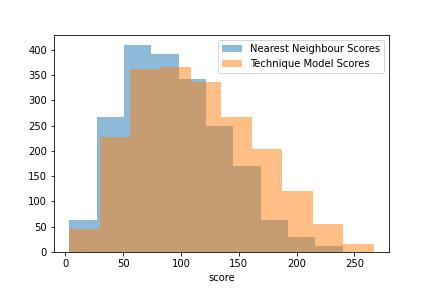
\includegraphics[width=0.8\linewidth]{technique_model_improvment}
\end{center}
   \caption{Score Distribution}
\label{fig:score_distribution}
\end{figure}

\begin{figure}
\begin{subfigure}
    \begin{left}
    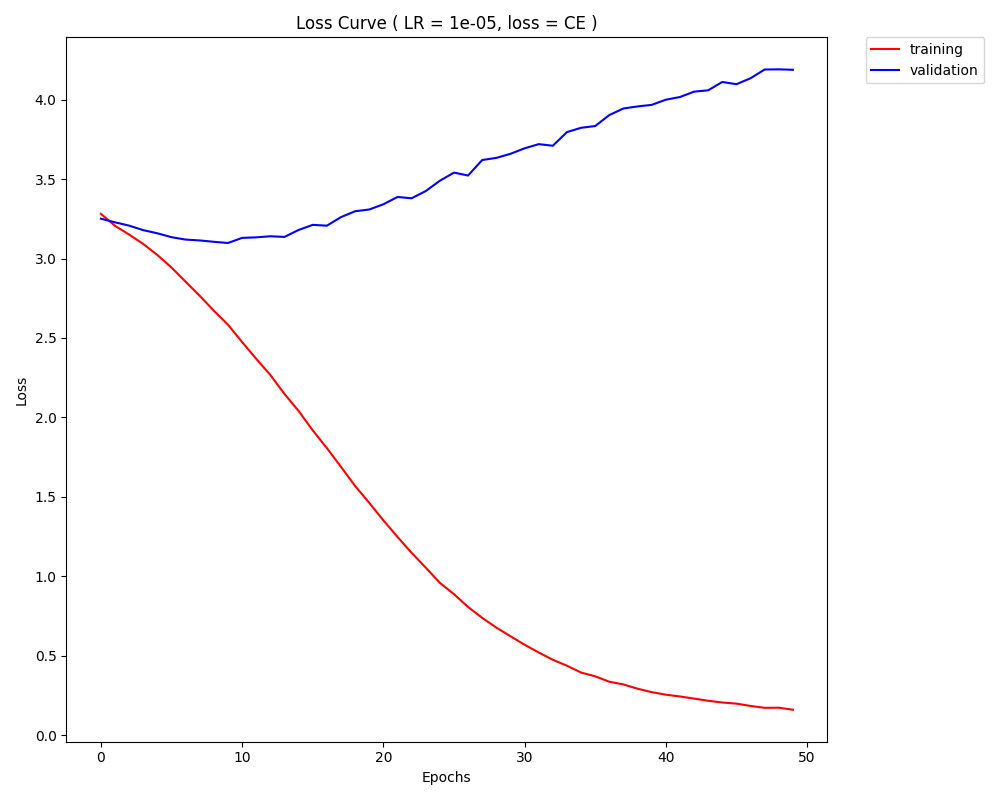
\includegraphics[width=0.45\linewidth]{lr_1e-05_e50_CE_loss_history}
    \end{left}
\end{subfigure}%
\begin{subfigure}
    \begin{right}
    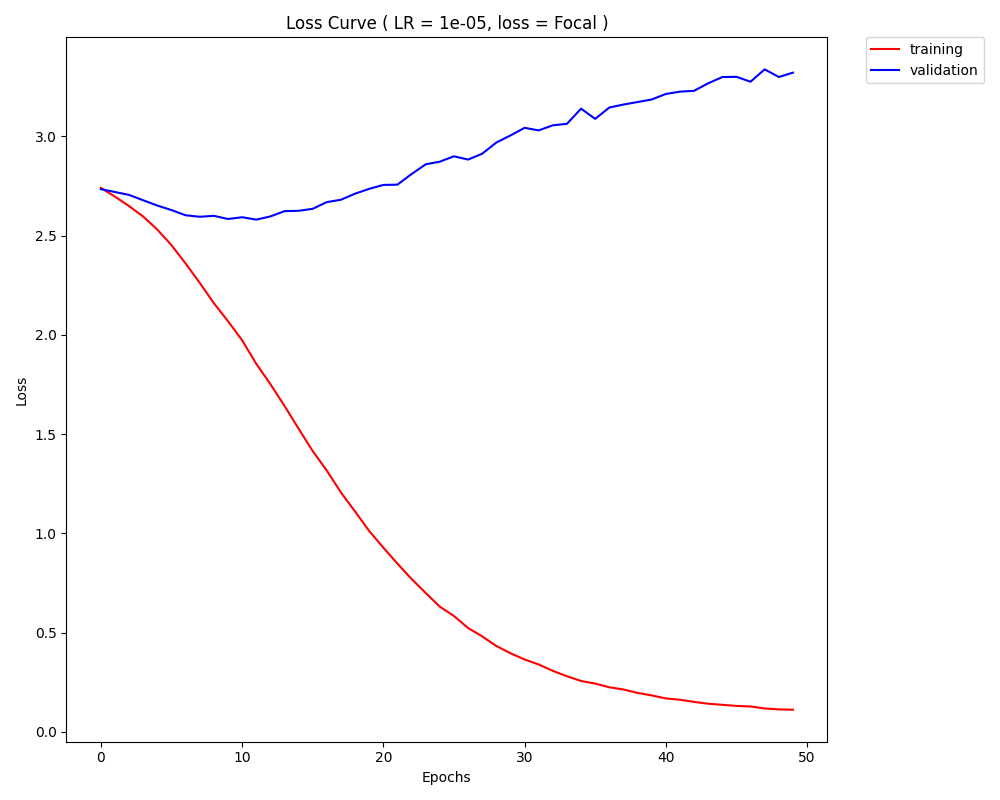
\includegraphics[width=0.45\linewidth]{lr_1e-05_e50_Focal_loss_history}
    \end{right}
\end{subfigure}%
  \caption{Category Loss Curves.}
\label{fig:category_loss_curve}
\end{figure}
\subsection{Food Category Classification}
The performance of the food category model follows the same precedence as the food technique model. For all experiments the model used a learning rate of $1e-05$ and Adam a the optimizing function. As stated above, the dataset being unbalanced requires us to utilize both the top-5 predicted categories and the per class accuracy. As stated above, the first iteration of the topic modeling used to generate categories output 200 unique categories. As shown in Table \ref{tab:category_accuracy}, filtering down the categories from 200 to 30 provided an improvement towards the model performance, but was still not able to solve the overfitting problem being seen. We than incorporated SMOTE in order to balance out the amount of images in each category. Once again, however, this did not solve the over fitting issue. 

The next experiment that was run was to compare the results between cross entropy loss and focal loss. Table \ref{tab:per_category_accuracy} shows the per category accuracy comparing both loss functions. While cross-entropy loss had a higher mean as seen in Table \ref{tab:category_accuracy}, it did not perform as well as focal-loss. Figure \ref{fig:category_loss_curve} further showcases this point. Both models experienced massive over fitting of the data, but the focal-loss function provided a lower overall loss through each epoch. In addition to that, Figure \ref{fig:category_accuracy_curve} shows the accuracy through each epoch using both loss functions. While though 50 epochs, the focal-loss modal performed roughly the same as the cross-entropy modal, it is clear that the former has an upward trend while the latter is starting to have a downward trend. This would mean with possibly better data representation, or more epochs the food category modal could show more improvement while utilizing focal-loss as the loss function. However, due to the massive over fitting being seen at training time, and the performance already achieved via the technique modal, we decided to not include the category modal into the overall nearest neighbor network. 

\begin{figure}
\begin{subfigure}
    \begin{left}
    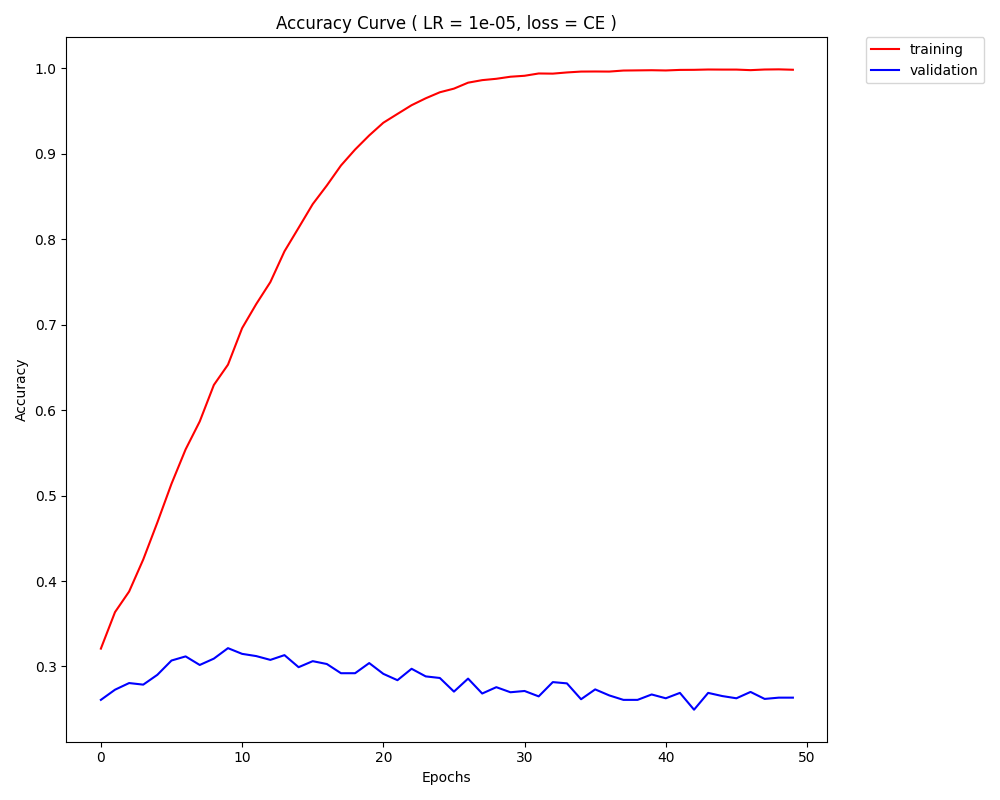
\includegraphics[width=0.45\linewidth]{lr_1e-05_e50_CE_accuracy_history}
    \end{left}
\end{subfigure}%
\begin{subfigure}
    \begin{right}
    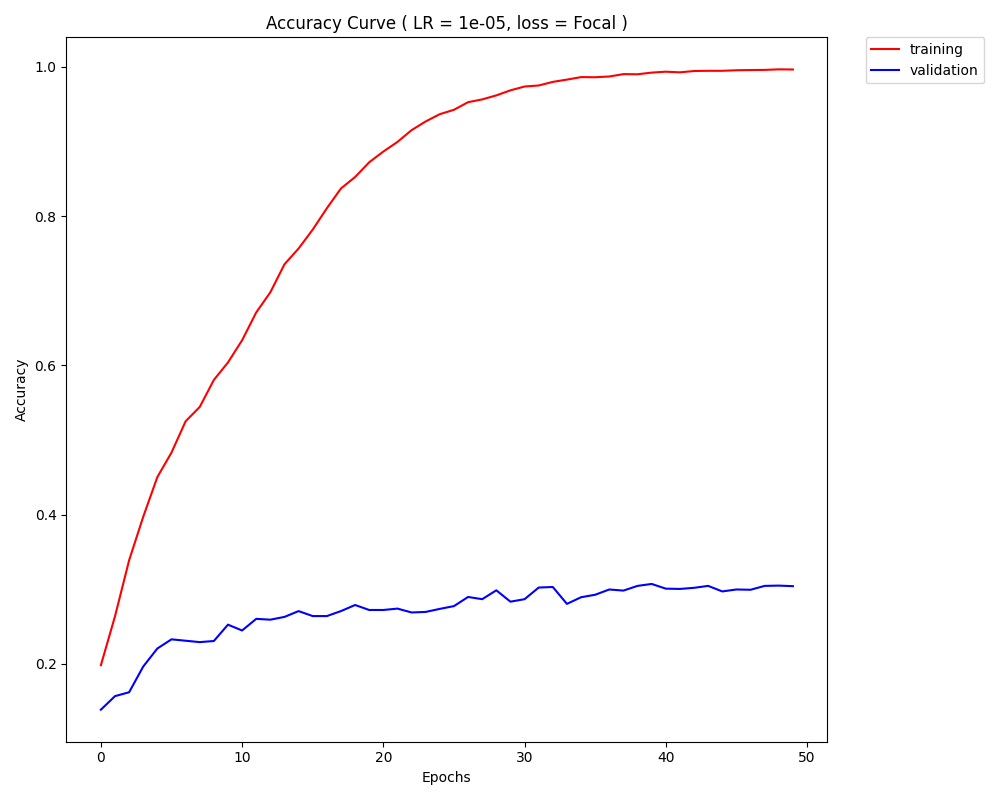
\includegraphics[width=0.45\linewidth]{lr_1e-05_e50_Focal_accuracy_history}
    \end{right}
\end{subfigure}%
  \caption{Category Accuracy Curves.}
\label{fig:category_accuracy_curve}
\end{figure}

%-------------------------------------------------------------------------



%-------------------------------------------------------------------------

\section{Work Division}

Please add a section on the delegation of work among team members at the end of the report, in the form of a table and paragraph description. This and references do \textbf{NOT} count towards your page limit. An example has been provided in eTable \ref{tab:contributions}.

\begin{table*}
\begin{center}
\begin{tabular}{|l|c|p{8cm}|}
\hline
Student Name & Contributed Aspects & Details \\
\hline\hline
Team Member 1 & Data Creation and Implementation & Scraped the dataset for this project and trained the CNN of the encoder. Implemented attention mechanism to improve results. \\
Team Member 2 & Implementation and Analysis & Trained the LSTM of the encoder and analyzed the results. Analyzed effect of number of nodes in hidden state.  Implemented Convolutional LSTM. \\
Karan Vohra & Implementation and Analysis & Implemented Food category model. Analyzed food category model results \\
Qimeng Wu & Data Creation, Implementation, and Analysis & Scraped the Food Technique dataset, trained the food technique model and analyzed the food technique model results.
\end{tabular}
\end{center}
\caption{Contributions of team members.}
\label{tab:contributions}
\end{table*}


\newpage
\newpage


%-------------------------------------------------------------------------
{\small
\bibliographystyle{ieee_fullname}
\bibliography{egbib}
}

\end{document}
